
\section{Interpreting Core}

\subsection{Example haskell program}

The example program is a simple hello world program. This may seem small, but making it
work requires quite alot of haskell functionality to be implemented.

\lstinputlisting[language=Haskell]{"../interpreter/tests/helloworld.hs"}

\subsection{Converted to Core}

As we can see, the simple hello world program becomes more complex when translated
to Core by ghc.

\lstinputlisting{"../interpreter/tests/helloworld.hcr"}

... TODO: Explain this representation in more detail.

\subsection{Converted to JSCore}

And translated to JSCore by our serializer:

\lstinputlisting{"../interpreter/tests/helloworld.hcj"}

\subsection{Parser}

Using the parsing libraries of pypy we can generate a nice graph from the result, 
see figure \ref{fig:helloworldgraph}

By simply traversing this datastructure we can generate the AST for the Core interpreter.

\begin{figure}
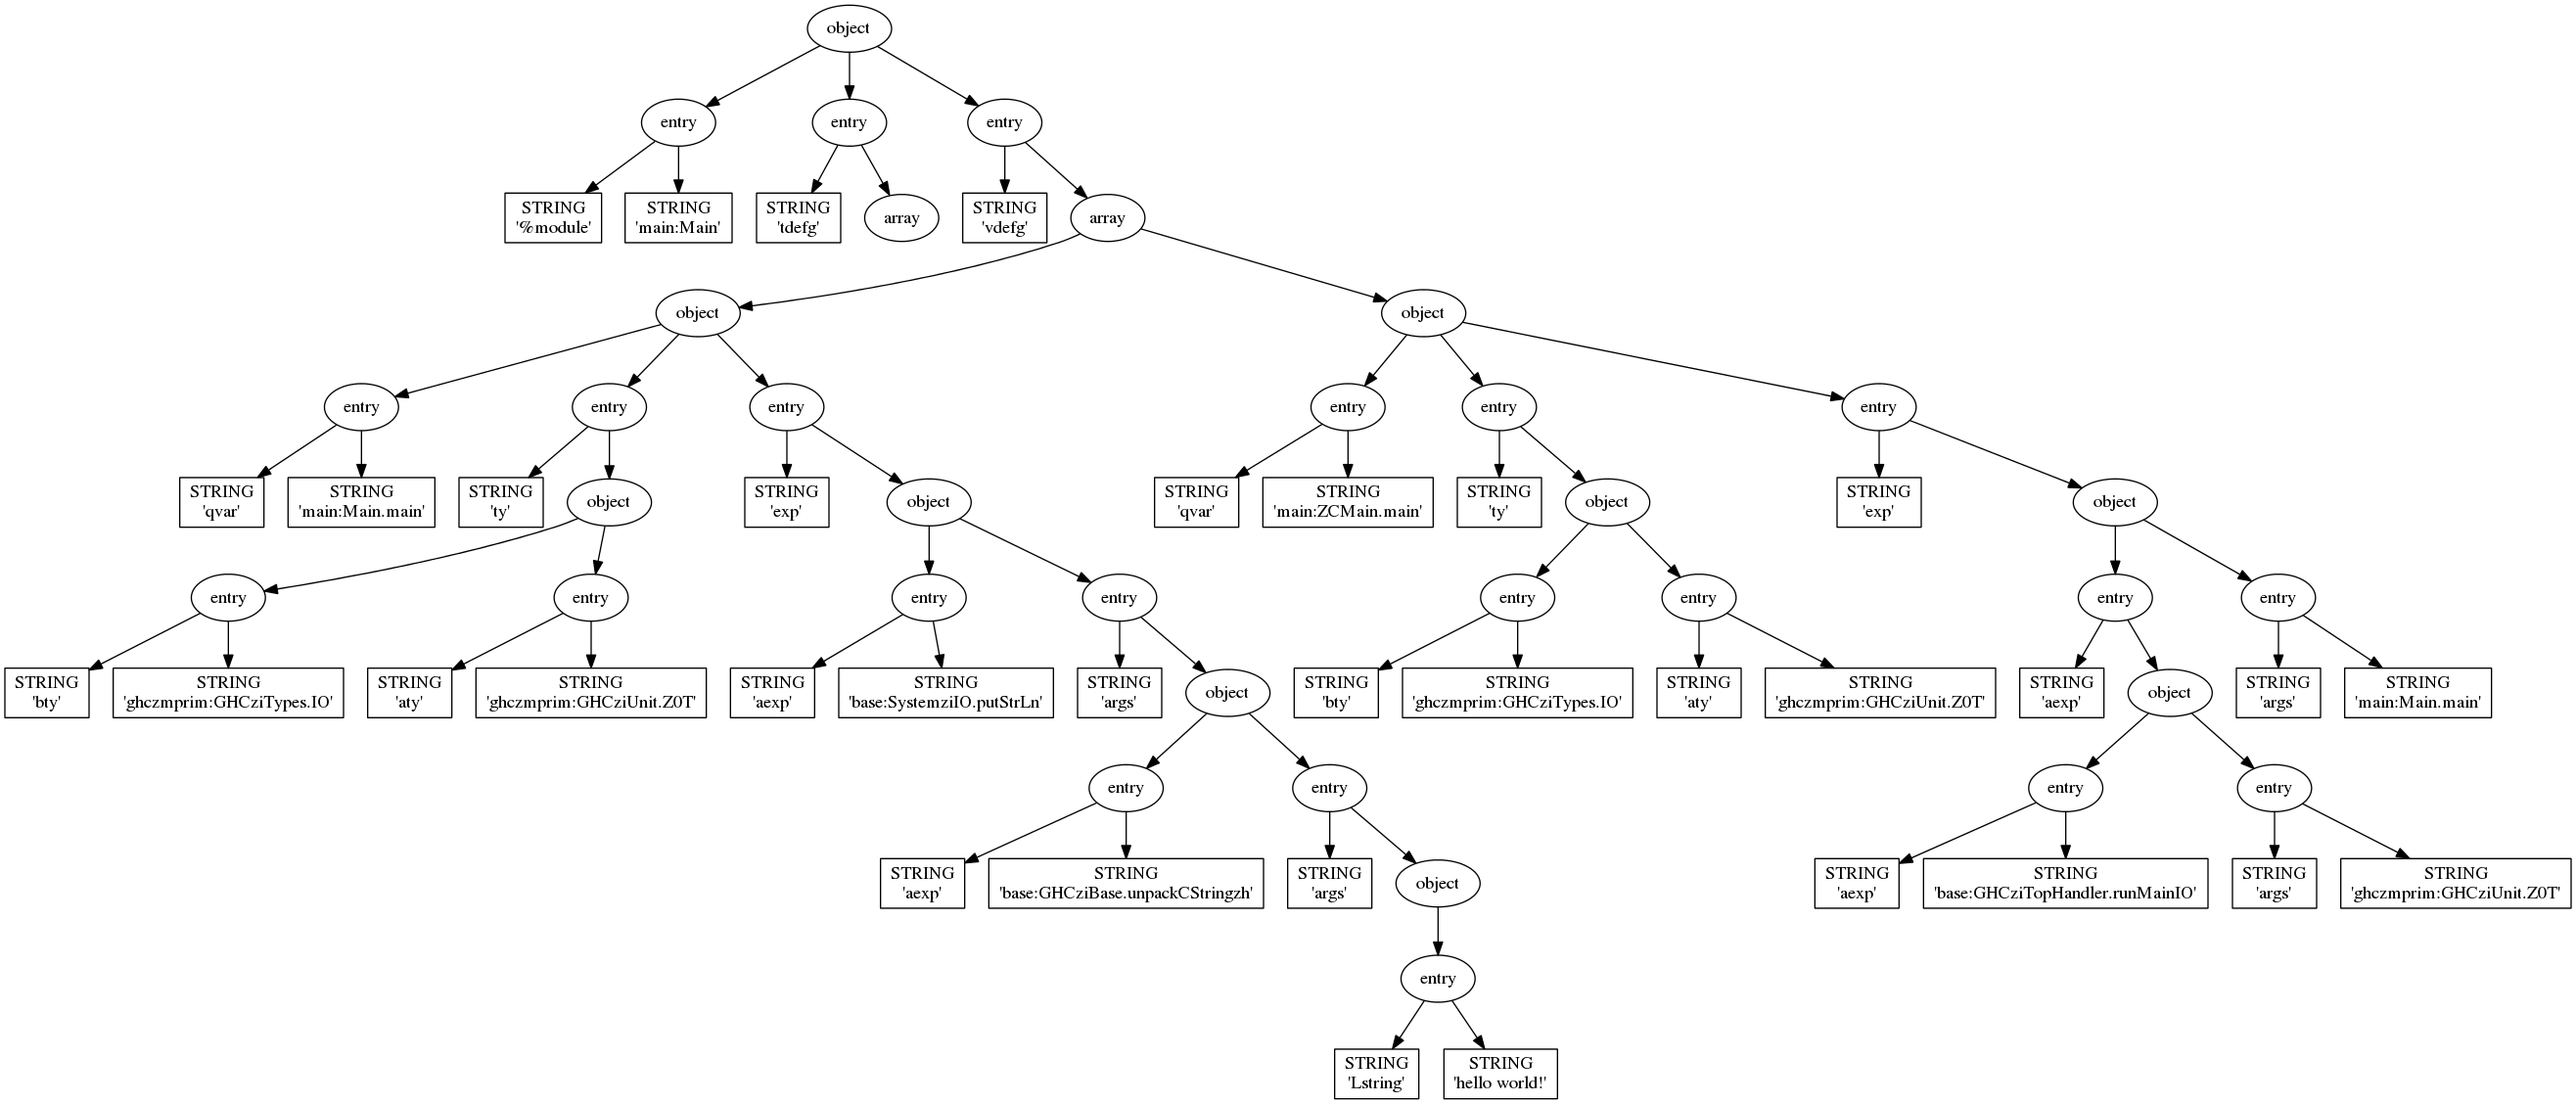
\includegraphics[width=\textwidth]{diags/helloworld2.png}
\caption{Example program translated to JSON}
\label{fig:helloworldgraph}
\end{figure}

\subsection{Compiler}

\subsubsection{Building the AST}


